This chapter discusses about the estimation of transformation model using matches estimated in previous chapter. The best matches we estimated still not guaranteed to be true matches, so there may be chances of getting wrong motion parameters if we include such false matches to estimate motion model. We use homography matrix as motion model for transformation. We use robust methods to estimate homography which uses only true matches.\\

\noindent If there is only translation or rotation between the images to be stitched, then stitching process will be simpler; we need only affine transformation parameters. The real problems will be to register images obtained using different camera angle; we have to estimate translation, rotation and projection parameters which can be represented by estimating \emph{homography matrix}.\\

\noindent A homography is a 3x3 matrix $H$ and the elements of the matrix contains the rotation, translation and projection parameters. We can change the value of homography $H$ without changing the projective transformation. Therefore, $H$ can be considered as homography matrix and it has 8 degrees of freedom (although it has 9 elements)~\cite{Dubrofsky:07}. In other words, we need to solve for 8 unknowns to get the homography matrix. 


\section{Algorithm for homography Estimation}
The homography matrix is solved using \emph{Direct Linear Transform (DLT)} algorithm if we have sufficient set of point correspondences. We solve the homography matrix by using the following equation:
\begin{equation}
x_i'=Hx_i
\label{eq:homography-estimation}
\end{equation}
where $x_i$ and $x_i'$ are 3 element vectors. For stitching problem, we use the corresponding points as vectors. In 2D problem, suppose, $\textbf{x}= (x,y,1)^T$ and $\textbf{x'}= (x',y',1)^T$ are two corresponding points, then the relationship will be
\begin{equation}
c\left(
\begin{array}{c}
	x \\
  y \\
	1	
\end{array}
\right)
=H \left( 
\begin{array}{c}
	x' \\
	y' \\
	1
\end{array}
\right)
\label{eq:homography-estimation-detail}
\end{equation}
Hartley and Zisserman~\cite{hartley:04} suggested to use a normalization step in DLT because the DLT algorithm is dependent on the origin and scale of co-ordinate system of the image. The normalized DLT algorithm can be summarized by the following steps:
\begin{enumerate}
	\item Translate the points such that the centroid lies at the origin. 
	\item The scaling of the points is carried out to maintain their average distance to be $\sqrt{2}$.
	\item Get transformations for both the images independently and apply DLT algorithm to get homography matrix. 
\end{enumerate}
For more detail algorithm, it is suggested to study chapter 4 of Hartley and Zisserman book~\cite{hartley:04}


\section{Robust Estimation}
\label{section:robust-estimation}
The homography estimation requires 4 corresponding points, and the matching methods described in previous sections are not robust i.e. there may be chances of some false correspondences. The two features in the images might not correspond to same the real feature. So, we need to identify the inlier and outlier correspondences and only inlier matches can be used for homography estimation. This section discusses two most popular methods for homography estimation.
%RANSAC%
\subsection{RANSAC}
\label{sec:ransac}
RANSAC (Random Sample Consensus) was first purposed by Fischler~\emph{et~al}~\cite{fischler:81} and it is the most commonly used robust estimation method for homographies~\cite{Dubrofsky:07}. This method selects 4 correspondences randomly and computes homography matrix $H$. Then other correspondences are classified as inliers or outliers depending on its concurrence with $H$. This process is repeated for a number of iterations and the iteration which gives largest number of inliers is identified. The homography $H$ for that iteration is chosen as the best transformation model.\\

\noindent The classification of inliers or outliers is carried out by assigning some distance threshold $t$ and if $\|\textbf{x'} - H\textbf{x}\| > t$, then the point is considered as outlier. The threshold value is problem specific. The higher the threshold value, the larger the inliers we get. Similarly, we choose a number of iterations $N$ so that at least one of the random samples will be free from outliers\footnote{We have to test each combination of random samples, so we need to limit the number of iterations}. Hartley and Zisserman~\cite{hartley:04} derived a formula to compute the number of iterations required for RANSAC:
\begin{equation}
N=log(1-p)/log(1-(1- \epsilon)^s)
\label{eq:number-of-iterations}
\end{equation} 
where $p$ = probability at least one of the samples is free from outlier. We generally use p=0.99\\
$\epsilon$=probability of outlier which can be expressed as 
\begin{equation}
\epsilon= 1- \frac{number\_of\_inliers}{total\_number\_of\_points}
\label{eq:outlier-probability}
\end{equation}
$s$ =number of correspondences used in each iteration. ($s=4$)\\

\noindent Hartley and Zisserman~\cite{hartley:04} \footnote{see comparison table in chapter 4 of the literature.} claims that if we have 5\% outliers(i.e. $\epsilon$=0.05) then only 3 iterations are needed to get at least one pure sample with probability=0.99.

%LMS%
\subsection{Least Median of Squares Regression}
\label{sec:least-median-square}
In RANSAC, we use distance threshold to identify outliers and exclude them for homography estimation. This method, as the name suggests, calculates the median of squares of the error value (i.e. difference between transformed and actual points) for each point in each iteration. The best homography is the one which gives least median value.\\

\noindent The Least median of Squares (LMS) was first introduced by Peter J. Rousseeuw~\cite{rousseeuw:84} and he claims that the estimator can resist the effect of nearly 50\% of contamination in the data. The ordinary least squares (OLS) estimators can not identify the non normal errors, so, LMS estimator is claimed to be a robust~\cite{rousseeuw:84}~\cite{onder:01} and it has the characteristics of being highly resistance to high proportion of outliers~\cite{onder:01}.\\

\noindent So, in summary, LMS is an effective method to detect the outliers. We do not need any initial parameters (unlike $t$ and $\epsilon$ in RANSAC). The only disadvantage of this method is that it can not work well if there are more than half outliers.  

\newpage
\section{Experimental Results}
% Select Ransac, because we are not sure that more than half of the keypoints are inliers
The first part of this section presents the result of RANSAC for homography estimation by identifying outliers. While LMS method (section~\ref{sec:least-median-square}) works good when there are more than 50\% inliers, it is not always guaranteed to have more than half accurate matches\footnote{there might be chances of being more false matches since we have used less accurate methods like SURF and ANN to get faster result}, so I prefer RANSAC method for robust estimation and it works even if there are large number of outliers. The equation~\ref{eq:number-of-iterations} reveals that we need few iterations to get a pure sample with high probability even if there are a lot of outliers.\\

\noindent In the next section, I include experiment on the effect of distance threshold value ($\sigma$) to the number of inliers or outliers.  The distance threshold $\sigma$ has been measured in pixels. 

\subsection{Robust Estimation with RANSAC}
For RANSAC, I have set the maximum possible number of iterations ($N$) up to 2000 and distance threshold ($\sigma$) 2 pixels. After some iterations, I got inliers (accurate matches), outliers (inaccurate matches) and the homography matrix $H$. Figure~\ref{fig:RANSAC-result} shows the inlier matches after I obtained using RANSAC method. From the figure, we can easily see that the all inliers are true matches.

\begin{figure}[H]%
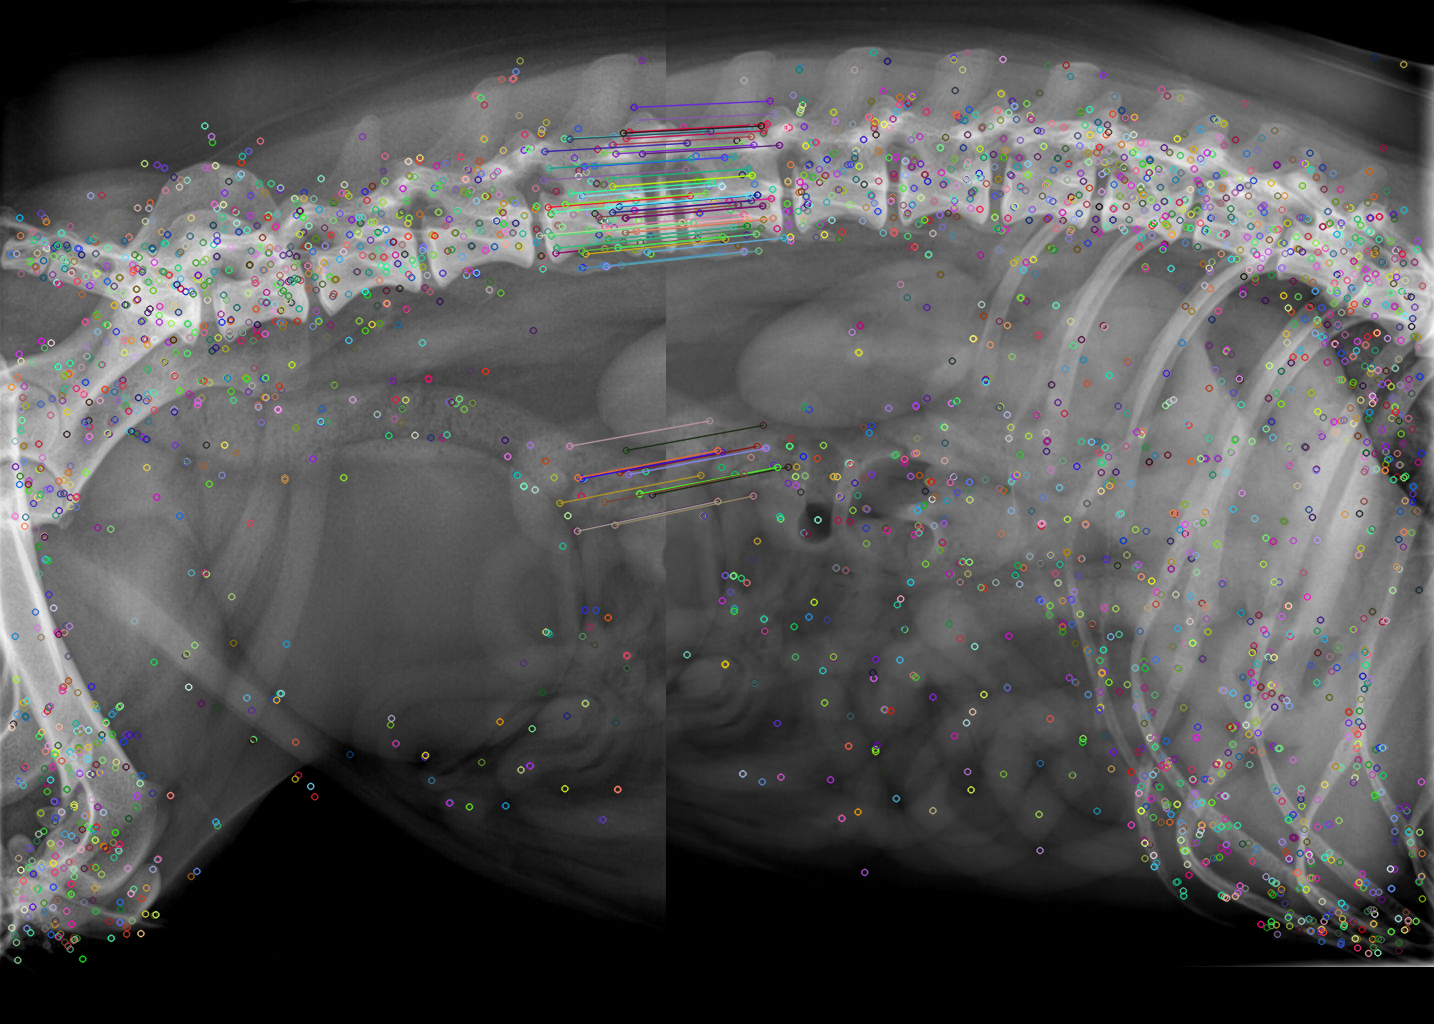
\includegraphics[scale=0.25]{2.mainmatter/2.Methodology/figures/inliers}
\caption[Matches After Removing Outliers]{Matches after removing outliers ($\sigma$=3 pixels). This figure shows all matches are accurate.}%
\label{fig:RANSAC-result}%
\end{figure}

\subsection{Effect of Distance Threshold ($\sigma$)}
The number of inliers is changed when we change the distance threshold $\sigma$. This section includes experiment on the effect of $\sigma$ to the number of inliers we obtained. The graph presented in figure~\ref{fig:inliers-vs-distance-threshold} shows that increase of $\sigma$, increases the number of inliers. So, we have to select proper $\sigma$ so that all inliers are true matches. With small possible value of $\sigma$=1 pixel, I got 50 inliers. Since the figure~\ref{fig:RANSAC-result} shows there are 62 accurate matches which implies that $\sigma$ = 1 is missing some true matches. The increase of $\sigma$ increases the inliers which also increases probability of including false matches as inliers. So, the best accepted values of $\sigma$ seems to be either 1 or 2. 

\begin{figure}[H]%
\centering
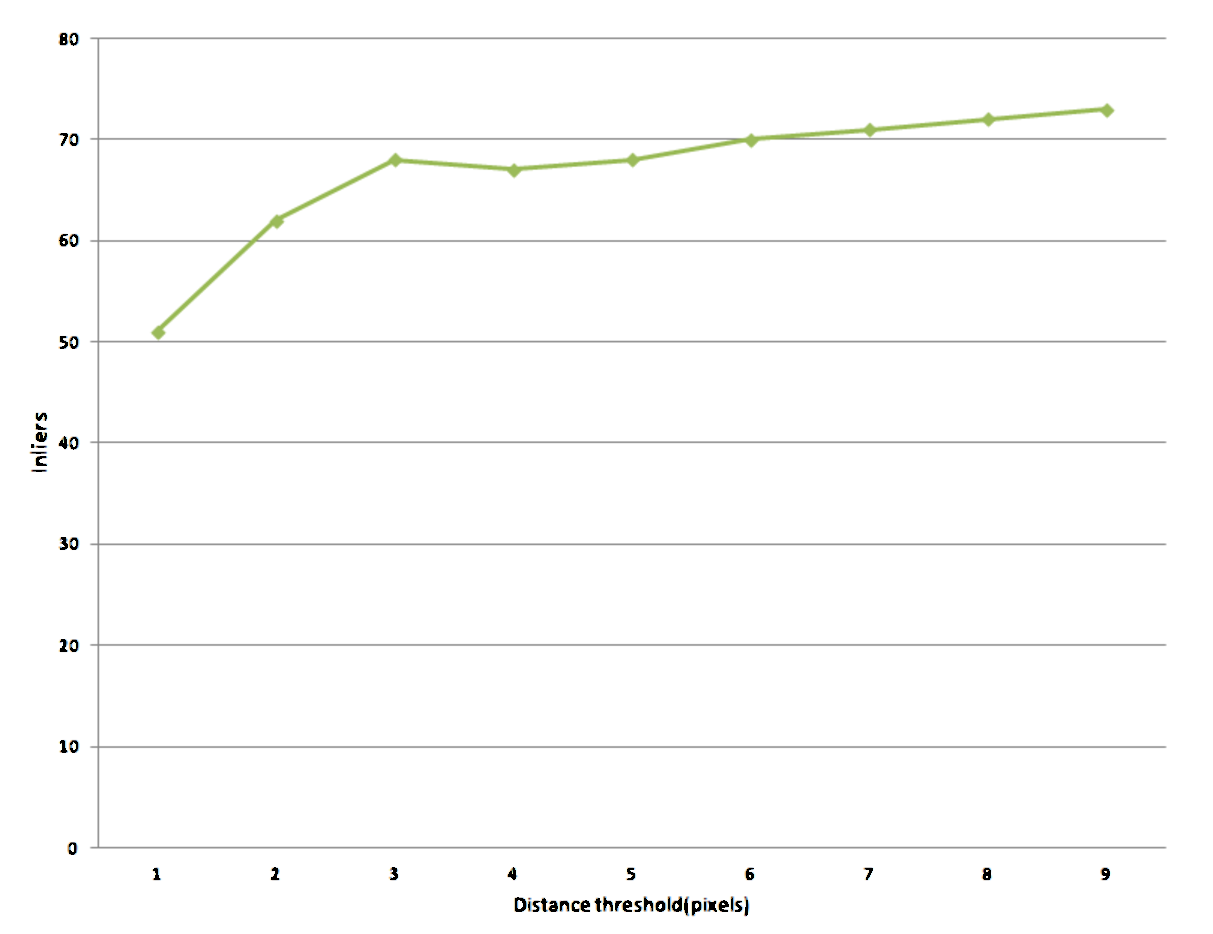
\includegraphics[width=1.0\columnwidth]{2.mainmatter/2.Methodology/figures/Inliers-threshold}%
\caption[Distance Threshold and Inliers Count]{Graph showing inliers versus distance threshold}%
\label{fig:inliers-vs-distance-threshold}%
\end{figure}

\noindent In some cases, if the stitching X-ray images are not exactly same, then key-points do not go with the transformation model (i.e. $H$) which results very few or sometimes insufficient inliers to guarantee the accuracy of homography. In that situation, we increase $\sigma$ value to get more inliers while estimating homography.\\

\noindent The number of inliers \footnote{The inliers in this context is the best inliers we got after a number of iterations.} can also be used to identify the feasibility of stitching between two images. There might be cases when we try stitching images which do not have any common region. The inliers are counted to confirm whether the images can be stitched. We define any number greater than sample size. Most of the time, if we have more than 15 inliers, we accept the homography to create composite image. For very few inliers\footnote{Few inliers imply limited or no overlapping between input images.}, there is chances of getting inaccurate homography and we stop the stitching process.



 


